\chapter{报告摘要}

本篇报告主要从任务需求分析、协议设计、协议实现和实验结果分析四个方面介绍了本次实验项目的实现过程,并通过第六章的个人总结综述了项目感悟。

在本次实验中,我们使用 C 语言和 socket 编程框架以及 HTML 前端网页、Python + pymysql 后端编程框架完成了一个能支持并发请求(测试在\ref{sec:apatest} 节)的具有注册、登陆功能的前后端综合项目 Liso Web Server。项目截图在 \ref{fig:3mains},图\ref{fig:laptop_main}展示了后端 Log 的基本情况。

\paragraph*{需求分析} 第二章分节介绍了该实验四周以及选做的任务以及相应目的和意义,起到开篇点题的作用。

\paragraph*{协议设计} 第三章协议设计主要从框架代码结构、数据结构设计以及诸如通信、消息解析、报文、流水线等关键结点切入,阐述了主要协议设计的思想,对程序运行的基本流程做了规范。

\paragraph*{协议实践} 第四章分功能地介绍了各个模块地实现办法。通过第四章的讲述,相信我们能够了解到整个程序模块化编程的思想以及各个模块在代码层面的实现办法。

\paragraph*{实验结果及分析} 第五章从 AutoLab 以及每周测试点的结果全方位地对项目进行了测试,并对比、验证了项目的鲁棒性与可扩展性。

\paragraph*{总结}该部分是对整个实验过程的总结和感悟。

\paragraph*{附录} 附录部分收录了一些实验截图。

\begin{figure}[htbp!]
    \begin{center}
        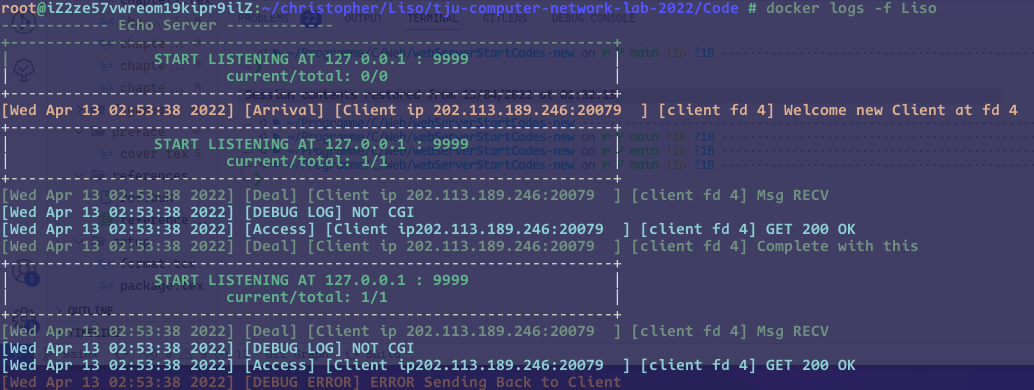
\includegraphics[height=1.5in]{liso_background1.png}
    \end{center}
    \caption{后端 Log 输出}\label{fig:laptop_main}
\end{figure}

